Debido a los resultados obtenidos en el problema del camino más corto estudiado anteriormente (\textit{sección~\ref{sec:5-primer_grafo}}), se decide aplicar las mismas pruebas sobre otro grafo con el mismo problema.

\begin{figure}[htbp]{fig:4-zhiqiang_grafo}{Grafo obtenido del \textit{artículo~\cite{solving_shortest_path_with_qaoa}}}
  \centering
  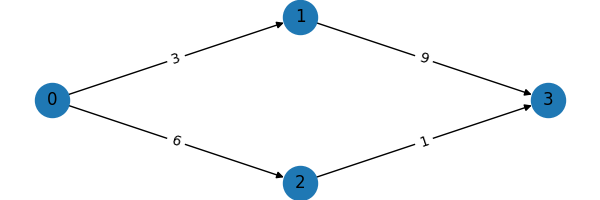
\includegraphics[scale=0.75]{zhiqiang-grafo/zhiqiang-grafo.png}
\end{figure}

Este grafo (\textit{figura~\ref{fig:4-zhiqiang_grafo}}) tiene la misma cantidad de nodos que el grafo~\ref{fig:4-primer_grafo} y una arista menos.
Esto se traduce en una aplicación de QAOA con menos restricciones pero con los mismos qubits. Con esta diferenciación se esperan obtener resultados que reproduzcan o corrijan el comportamiento dado con el grafo anterior al aumentar el número de capas.

\begin{itemize}
\item \textbf{Objetivo:}

  \begin{align*}
    &\min(3X_{01} + 6X_{02} + 9X_{13} + 1X_{23}) \\
    &\textnormal{dde } X_{ij} = \begin{cases}
      1 \textnormal{ si el camino contiene la arista del nodo \textit{i} al \textit{j}} \\
      0 \textnormal{ en otro caso}
    \end{cases}
  \end{align*}

\item \textbf{Restricciones:}

  \begin{enumerate}
  \item $X_{01} + X_{02} = 1$: Equivalente a la \textit{restricción~\ref{it:4-primer_grafo_restriccion_ini}} del problema previo.
  \item $X_{01} = X_{13} \\
    X_{02} = X_{23}$: Equivalentes a las \textit{restricciones~\ref{it:4-primer_grafo_restriccion_inter}} del problema previo.

  \item $X_{13} + X_{23} = 1$:  % TODO: Añadir explicación
    % TODOOO: Tal vez hacerlo quitando esta restricción???

  \end{enumerate}

  Con el fin de mantener las similitudes con el problema anterior se elige el modificador de Lagrange (\textit{P}) utilizando la misma métrica, a saber:
  $P > \max_{x}{f_{\textnormal{sin restricc}}(x)} = \sum_{(i, j)\in{E}}{w_{ij}} = 19$. Por este motivo se escoge $P = 20$
\end{itemize}

Al añadir las restricciones, como se explica en la \textit{sección~\ref{sec:3-problemas de optimizacion combinatoria}}, la función de coste definitiva en formato QUBO queda como:

\begin{align*}
  f(X) &= 3X_{01} + 6X_{02} + 9X_{13} + 1X_{23} + \\
       &+ P{(X_{01} + X_{02} - 1)}^2 + P{(X_{13} + X_{23} - 1)}^2 + P{(X_{01} - X_{13})}^2 + P{(X_{02} - X_{23})}^2
\end{align*}

Para el paso de la función de la versión QUBO a versión Ising se debe realizar un cambio de variable $X_{ij} \rightarrow \frac{1 - z_k}{2}$. Con este paso se hará que, como las variables $X_{ij}$ toman valores $\{0, 1\}$, las variables $z_k$ tomen valores $\{-1, 1\}$. Además cada variable $z_k$ corresponderá al qubit \textit{k}-ésimo. La correspondencia entre variables $X_{ij}$ y $z_k$ es la siguiente:
$X_{01}$ corresponde con $z_0$,
$X_{02}$ corresponde con $z_1$,
$X_{13}$ corresponde con $z_2$ y
$X_{23}$ corresponde con $z_4$.

Al igual que para los problemas anteriores, y de acuerdo con la sección  % TODO: Citar
cada variable $z_i$ corresponde a un operador Pauli-Z en el qubit $i$.

La versión Ising de la función de coste queda de esta forma:\footnote{Dado $z_i \in \{-1, 1\}$, se cumple $z_i^2 = 1$}

\begin{align*}
  g(z) &= 3\frac{1 - z_0}{2} + 6\frac{1 - z_1}{2} + 9\frac{1 - z_2}{2} + 1\frac{1 - z_3}{2} + \\
       &+ P{(\frac{1 - z_0}{2} + \frac{1 - z_1}{2} - 1)}^2 + P{(\frac{1 - z_2}{2} + \frac{1 - z_3}{2} - 1)}^2 + \\
       &+ P{(\frac{1 - z_0}{2} - \frac{1 - z_2}{2})}^2 + P{(\frac{1 - z_1}{2} - \frac{1 - z_3}{2})}^2 = \\
  = &  -1.5z_0 - 3z_1 - 4.5z_2 - 0.5z_3 + \\
       &+ 10*(z_0z_1 - z_0z_2 - z_1z_3 + z_2z_3) + 49.5
\end{align*}

El \textbf{problem hamiltonian} (descrito en la \textit{sección~\ref{sec:3-circuito de qaoa}}) partiendo de $g(z)$ es:

\begin{align*}
  &U(C, \gamma) = \exp(-i \gamma C) = \\
  &= Rz_0(-1.5 * 2\gamma) \cdot Rz_1(-3 * 2\gamma) \cdot Rz_2(-4.5 * 2\gamma) \cdot Rz_3(-0.5 * 2\gamma) \cdot \\
  &\cdot Rz_0z_1(10 * 2\gamma) \cdot Rz_0z_2(-10 * 2\gamma) \cdot Rz_1z_3(-10 * 2\gamma) \cdot Rz_2z_3(10 * 2\gamma)
\end{align*}

Con el \textbf{mixing hamiltonian} y el vector inicial, definidos en la \textit{sección~\ref{sec:3-circuito de qaoa}} y el \textbf{problem hamiltonian} obtenido se puede construir el circuito cuántico.

\begin{figure}[htbp]{fig:4-zhiqiang_circuito}{ Circuito obtenido ($p=1$) }
  \centering
  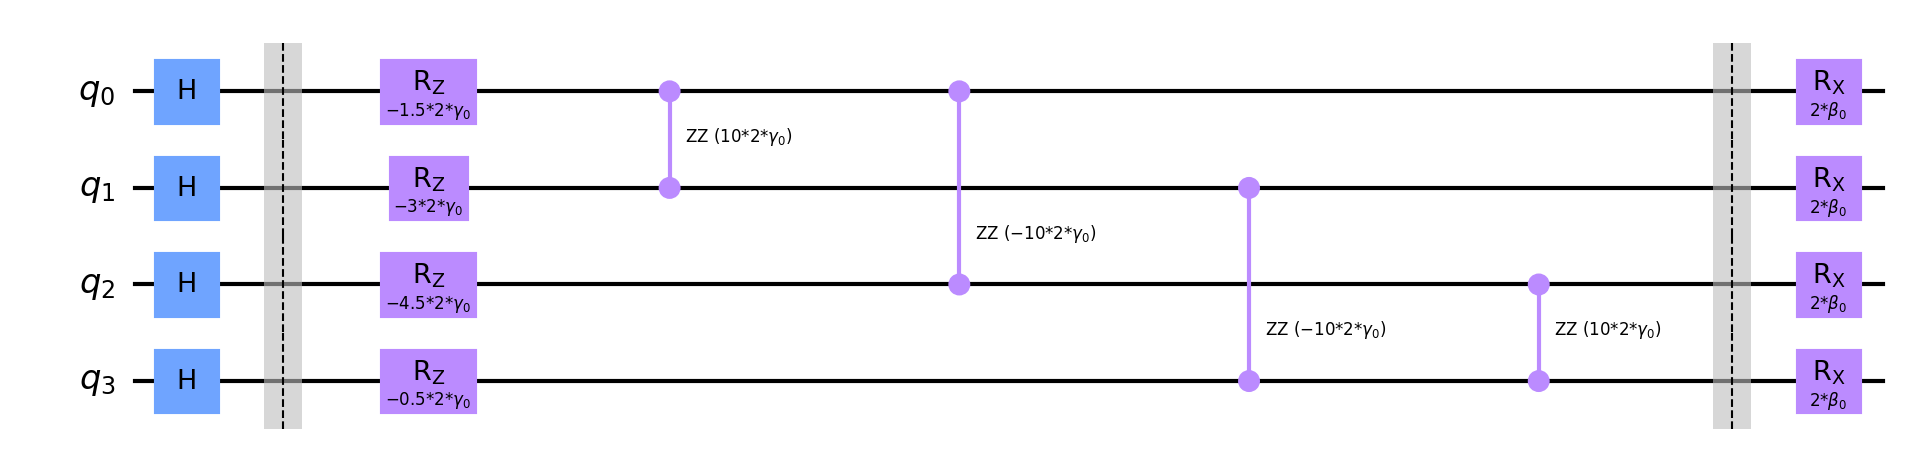
\includegraphics[scale=0.27]{circuits/zhiqiang/zhiqiang-circuit-p1-var.png}
\end{figure}

En el artículo del que se ha obtenido el problema no se muestra la construcción del circuito de QAOA, por lo que el resultado obtenido en la \textit{figura~\ref{fig:4-zhiqiang_circuito}} no puede ser comparado.

%%% Local Variables:
%%% mode: latex
%%% TeX-master: "../tfgtfmthesisuam"
%%% End:
